%----------------------------------------------------------------------------------
% Exemplo do uso da classe tcc.cls. Veja o arquivo .cls
% para mais detalhes e instruções.
%----------------------------------------------------------------------------------

% Seleção de idioma da monografia. Por enquanto as únicas opções
% suportadas são 'portuguese' e 'english'
% Para impressão em frente e verso, use a opção 'twoside'. Da
% mesma forma, use 'oneside' para impressão em um lado apenas.
\documentclass[portuguese,oneside]{tcc}

%----------------------------------------------------------------
% Coloque seus pacotes abaixo.
%
% Obs.: muitos pacotes de uso comum do LaTeX, como amsmath,
% geometry e url já são automaticamente incluídos pela classe
% (veja o arquivo .cls). Isso torna obrigatória a presença destes
% no sistema para o uso desta classe, mas ao mesmo tempo o uso se
% torna mais simples.  Recomendo a instalação da versão mais
% recente da distribuição TeXLive (para Windows e UNIXes):
% www.tug.org/texlive/
%
% Pacotes e opções já incluídas automaticamente:
%
% \RequirePackage[T1]{fontenc}[2005/09/27]
% \RequirePackage[utf8x]{inputenc}[2008/03/30]
% \RequirePackage[english,brazil]{babel}[2008/07/06]
% \RequirePackage[a4paper]{geometry}[2010/09/12]
% \RequirePackage{textcomp}[2005/09/27]
% \RequirePackage{lmodern}[2009/10/30]
% \RequirePackage{indentfirst}[1995/11/23]
% \RequirePackage{setspace}[2000/12/01]
% \RequirePackage{textcase}[2004/10/07]
% \RequirePackage{float}[2001/11/08]
% \RequirePackage{amsmath}[2000/07/18]
% \RequirePackage{amssymb}[2009/06/22]
% \RequirePackage{amsfonts}[2009/06/22]
% \RequirePackage{url}
% \RequirePackage[table]{xcolor}[2007/01/21]
%----------------------------------------------------------------
% Para inserção de figuras.
\usepackage{graphicx}
% Utilize a opção 'pdftex' se você estiver usando o pdflatex (que
% permite figuras em formatos como .jpg ou .png)
%\usepackage[pdftex]{graphicx}

% Para tabelas com elementos ocupando mais de uma linha
\usepackage{multirow}
% Para frações na mesma linha (ex. ⅓).
\usepackage{nicefrac}
% Para inserir figuras lado a lado.
% \usepackage{subfigure}
% Para formatar algoritmos.
% A opção [algo2e] é necessária para evitar conflitos
% com as definições da classe.
%\usepackage[ruled, algo2e, linesnumbered]{algorithm2e}
%\usepackage{algorithmic}
% Um float do tipo algoritmo. No momento
% este pacote é incompatível com a classe.
%\usepackage{algorithm}
\usepackage{todonotes}
\usepackage{pgfgantt}
\usepackage{algpseudocode}
\usepackage{algorithm}
\newcommand\frm[2][noinline]{\todo[size=\tiny,author=Felipe,color=red!75,#1]{#2}}
\newcommand{\msr}[1]{\todo[color=blue!50,author=Matheus]{#1}}
%----------------------------------------------------------------
% Autor (OBRIGATÓRIO)
%----------------------------------------------------------------
\author{Matheus de Souza Redecker}

%----------------------------------------------------------------
% Título (OBRIGATÓRIO). Devem ser passados DOIS parâmetros,
% o título em português E o inglês, não importando o idioma
% escolhido. Os títulos são utilizados para a montagem da capa,
% resumo e abstract mais tarde.
%----------------------------------------------------------------
\title{Adversarial Hierarchical-Task Network integrado com aprendizado por reforço para jogos em tempo real}
      {Adversarial Hierarchical-Task Network integrated with reinforcement learning for Real-Time Games}

%----------------------------------------------------------------
% Opções para o tipo de trabalho (OBRIGATÓRIO)
%----------------------------------------------------------------
\tipotrabalho{\ptci}         % Proposta de Trabalho de Conclusão
%\tipotrabalho{\tci}         % Trabalho de Conclusão I
%\tipotrabalho{\tcii}        % Trabalho de Conclusão II

%----------------------------------------------------------------
% Seleção do curso ("este trabalho é um requisito parcial para
% obtenção do grau de (mestre ou doutor) em Ciência da Computação").
%----------------------------------------------------------------
\curso{\cc} % Ciência da Computação
%\curso{\si} % Sistemas de Informação
%\curso{\es} % Engenharia de Software

%----------------------------------------------------------------
% Orientador (e Co-orientador, caso haja um). É OBRIGATÓRIO
% informar pelo menos o orientador.
%----------------------------------------------------------------
\orientador{Felipe Rech Meneguzzi}
%\coorientador{Ciclano de Farias}

%----------------------------------------------------------------
% A capa é inserida automaticamente. Por isso não é necessário
% chamar \maketitle
%----------------------------------------------------------------
\begin{document}

%----------------------------------------------------------------
% Depois da capa vem a dedicatória e a epígrafe.
%----------------------------------------------------------------
%\dedicatoria{Dedico este trabalho a meus pais.}

%\epigrafe{The art of simplicity is a puzzle of complexity.}
         %{Douglas Horton}

%----------------------------------------------------------------
% Também dá para fazer as duas na mesma página:
%----------------------------------------------------------------
%\dedigrafe{Dedico este trabalho a meus pais.}
%          {The art of simplicity is a puzzle of complexity.}
%          {Douglas Horton}

%----------------------------------------------------------------
% A seguir, a página de agradecimentos (OPCIONAL):
%----------------------------------------------------------------
%\begin{agradecimentos}
%.
%\end{agradecimentos}

%----------------------------------------------------------------
% Resumo, com as palavras-chave passadas por parâmetro
% (OBRIGATÓRIO, ao menos para teses e dissertações)
%----------------------------------------------------------------
\begin{resumo}{planejamento, HTN, busca adversária, aprendizado por reforço}
Jogos de estrategia em tempo real são difíceis ao ponto de vista da IA, por conta do grande espaço de estados, e ainda a limitação do tempo para tomar uma ação. Uma alternativa é combinar busca adversaria com técnicas de HTN, o algoritmo é chamado de \textit{Adversarial Hierarchical-Task Network}. Para tentar melhorar o desempenho do algoritmo é proposto uma unificação do algoritmo com técnicas de aprendizado por reforço. Para validar é utilizado o jogo MicroRTS como plataforma. 
\end{resumo}

%----------------------------------------------------------------
% Abstract, com as palavras-chave passadas por parâmetro
% (OBRIGATÓRIO, ao menos para teses e dissertações)
%----------------------------------------------------------------
\begin{abstract}{planning, HTN, adversal search, reinforcement learning}
Real-time strategy games are hard from IA view, because of the high amount of states spaces and have a short time to choose actions. An alternative is join adversarial search techniques with HTN techniques, the algorithm is called Adversarial Hierarchical-Task Network. To improve the performance, is proposed the join of this algorithm with reinforcement learning techniques. The game used as platform is MicroRTS.
\end{abstract}

%----------------------------------------------------------------
% Listas e sumário, nessa ordem. Somente o sumário é obrigatório,
% portanto, comente as outras listas, caso sejam desnecessárias.
%----------------------------------------------------------------
\listoffigures       % Lista de figuras      (OPCIONAL)
%\listoftables        % Lista de tabelas      (OPCIONAL)
\listofalgorithms    % Lista de algoritmos   (OPCIONAL)
\listofacronyms      % Lista de siglas       (OPCIONAL)
%\listofabbreviations % Lista de abreviaturas (OPCIONAL)
%\listofsymbols       % Lista de símbolos     (OPCIONAL)
\tableofcontents     % Sumário               (OBRIGATÓRIO)

%----------------------------------------------------------------
% Aqui começa o desenvolvimento do trabalho. Para uma melhor
% organização do documento, separe-o em arquivos,
% um para cada capítulo. Para isso, utilize o comando \include,
% como mostrado abaixo.0
%----------------------------------------------------------------

\sigla{IA}{Inteligência Artificial}
\sigla{HTN}{Hierarchical Task Network}
\sigla{AHTN}{Adversarial Hierarchical Task Network} 
\sigla{RTS}{Real-time Strategy}

%!TEX root = proposta.tex 
%% Matheus renomeia "exemplo.tex" para um nome mais descritivo (e muda a linha acima)
\chapter{\label{chap:intro}Introdução}

Inteligencia artificial(IA) é uma área em ciência da computação que tem como objetivo fazer com que o computador seja capaz de realizar tarefas que precisam ser pensadas, como é feito pelas pessoas.  
A IA possui algumas áreas de aplicação, tais como: aprendizado, planejamento, jogos, e mineração de dados entre outras. 

%A utilização de IA para jogos começou simples, com a aplicação de técnicas para jogos como xadrez e jogo da velha, mas atualmente é difícil encontrar um jogo que não utilize alguma técnica de IA.\frm{Quem disse isto? Citação ou não existiu.} 
As técnicas de IA utilizadas nos jogos são necessárias para conseguir uma melhor interação com o jogador, tornando o jogo mais real e assim prendendo a atenção do jogador \cite{millington2009artificial}. 
As técnicas utilizadas nos jogos, geralmente, são mais simples do que as que utilizadas no meio acadêmico, pelo fato de que o tempo de resposta dos algoritmos é superior ao tempo que se tem para tomar uma ação ótima dentro do jogo \cite{intelligence2003modern}. 
Nos jogos as reações devem ser quase que imediatas, para isso técnicas que tentam explorar todo o espaço de estados do jogo se tornam inviáveis para jogos mais complexos.
Por exemplo, no xadrez a quantidade aproximada de estados possíveis é de $10^{40}$, isso mostra que o poder de processamento para gerar, de maneira rápida, uma ação precisa ser alto \cite{millington2009artificial}. Então é difícil conseguir gerar uma ação ótima, em alguns casos são gerados ações sub ótimas para que o tempo de resposta não seja muito alto \cite{intelligence2003modern}.     %\frm{Tá, agora tu tens que concluir alguma coisa... Então é complicado gerar uma ação ótima, e daí?}


%\frm[inline]{De repente falar de busca adversária antes, ou algo assim. Eu sei que tu tens que conectar estas idéias.}
A busca é utilizada, dendo da IA, para achar a possível sequencia de ações que resolve um problema, considerando varias possibilidades de sequencia dessas ações. Os algoritmos de busca se diferenciam entre si na forma de escolher qual o próximo estado na busca pelo objetivo. Já busca adversária é utilizada para a resolução de problemas de busca em modo competitivo. A busca adversária pressupõe que sempre o oponente irá realizar sempre a jogada que mais lhe beneficia, isso nem sempre acontece, seja porque o jogador é iniciante ou comete um erro. O ser humano consegue raciocinar para decidir as ações, mas nem sempre ele é otimizador perfeito, ele consegue ser muito bom, mas o modo de pensar não o torna perfeito sempre. Planejamento é uma área da IA que busca a geração de planos de forma automática, parecido com a busca, utiliza técnicas para buscar a geração de um plano que satisfaça um objetivo. A utilização de técnicas de planejamento em jogos é uma tarefa difícil devido a sua grande quantidade de ações possíveis. Esse gênero de jogo possui um fator de ramificação muito grande, e cresce exponencialmente, com isso aplicar algoritmos de planejamento se torna uma tarefa não trivial \cite{intelligence2003modern}. 


%\frm{Tu conectaste as idéias melhor no abstract, aqui tu terias que introduzir algo no sentido de que: para mitigar as limitações de eficiência computacional de abordagens tradicionais de raciocínio em jogos, X e Y propuseram o AHTN}
Na busca de mitigar as limitações de eficiência computacional de abordagens tradicionais de raciocínio em jogos, Santiago Ontanõn e Michael Buro propuseram o algoritmo chamado \textit{Adversarial Hierarchical Task Network (AHTN)} \cite{ontanon2015adversarial}. Neste algoritmo são combinadas técnicas de HTN com o algoritmo de busca adversaria \textit{minimax search}. 

Propomos a utilização do algoritmo AHTN combinado com uma técnica de aprendizado por reforço em um jogo de estrategia em tempo real combinando uma técnica de aprendizado por reforço. Com este trabalho pretendemos apresentar que o algoritmo de AHTN apresenta melhores resultados quando aplicado junto com técnicas de aprendizado por reforço.



%Para resolver esse problema existe uma proposta de solução utilizando o algoritmo de AHTN \cite{ontanon2015adversarial}.\frm{Jargão} Para melhor o desempenho desse algoritmo, proponho uma união desse algoritmo com um algoritmo de aprendizado de maquina através da ferramenta WEKA. \frm[inline]{A ferramenta que tu usa, neste ponto, é irrelevante. Seja simples e direto para dizer o que tu queres fazer.}

%\begin{itemize}
%\item introdução de IA
%\item linkar IA a jogos
%\item dificuldades de aplicação em jogos
%\item motivação 
%\end{itemize}
%!TEX root = proposta.tex 
%% Matheus renomeia "exemplo.tex" para um nome mais descritivo (e muda a linha acima)
\chapter{\label{chap:conte}Contexto}

\todo[color=red,author=Felipe,inline]{Ok, aqui está bem genérico, agora começa a projetar parágrafo por parágrafo do material que tu já leste (bullets para cada parágrafo), e me manda depois que tu completares o texto. Deixa as bullets no topo para eu entender o teu raciocínio}

\section{Planejamento} 

Planejamento é o modo racional de agir. Planejamento é a geração de um plano para atingir um objetivo. O processo do planejamento consistem em escolher e gerenciar as ações, antecipando os resultados a fim de atingir um objetivo pré definido \cite{ghallab2004automated}. \\
Para que alguns objetivos consigam ser alcançados, as ações que são tomadas não necessariamente necessitam de um planejamento, nas atividades do dia-a-dia a maioria das ações que são tomadas não são planejadas. Para fazer um planejamento é avaliado os ganhos de planejar as ações em vista do objetivo, geralmente, os planos nem sempre são os melhores possíveis, pois a busca de planos considerados perfeitos são mais demorados para construir, fazendo com que planos razoáveis ou bons sejam escolhidos ao invés dos perfeitos \cite{ghallab2004automated}. \\
Pelo fato de se ter alguns tipos de ações, também há alguns formas de planejamento \cite{ghallab2004automated}. Algumas das formas de planejamento são:

\begin{itemize}
	\item Planejamento de trajetória e movimento - Este tipo de planejamento foca em problemas onde é preciso simplificar um caminho de um ponto inicial a um objetivo e ainda controlar a trajetória através do caminho. Por exemplo, gerar a rota de um caminhão e movimento de um braço mecânico. 
	\item Planejamento de percepção - Este tipo de planejamento é focado em problemas onde os planos devem se preocupar com as informações obtidas pelo sistema. Por exemplo,  a construção de um ambiente virtual de uma área urbana através de imagens. 
	\item Planejamento de navegação - Combina os dois tipos acima de planejamento, de percepção e movimento, para problemas que precisem da combinação de localizações e percepções. Por exemplo, andar por um rio desviando de obstáculos.  
\end{itemize}

Planejamento na computação é a área da Inteligencia Artificial(IA) que busca a geração de planos automaticamente de forma computacional \cite{ghallab2004automated}. E para representar o processo de planejamento no computador é preciso de um modelo conceitual que é um recurso teórico usado para descrever o problema de forma geral e assim podendo aprofundar dependendo da abordagem. Como planejamento é  focado na escolha de ações para acontecer mudança de estados no sistema, o modelo para descrever esse processo deve ser dinâmico, ou seja, que permita a mudança do ambiente\cite{ghallab2004automated}. \\

O modelo geral utilizado para representar um plano é o \textit{state-transition systems}. O modelo é representado por $\sum = (S, A, E, \gamma) $. Onde S representa os estados, A as ações, E os eventos que podem ocorrer no sistema, e $\gamma$ a função de transição composta por $ \gamma: S \times A \times E \rightarrow S'$. A figura \ref{fig:planmodelo} mostra uma representação desse modelo \cite{ghallab2004automated}.


\begin{figure}[ht]
	\centering
	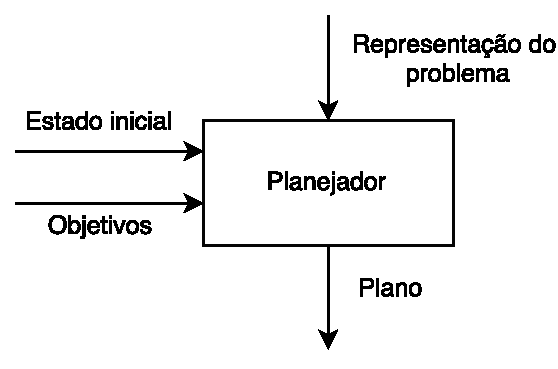
\includegraphics[width=0.4\textwidth]{fig/modelo.pdf}
	\caption{Modelo de estado e transição}
	\label{fig:planmodelo}
\end{figure} 

Um plano é gerado, quando dado um estado inicial e um objetivo, um conjunto de ações é gerado e quando executadas levam ao objetivo. O processo usado para conseguir isso é chamado de planejamento, onde é necessário ter uma descrição do sistema($\sum$) onde os estados e as ações são definidos.\\ 
Os estados são representados por um conjunto de átomos sem função \cite{intelligence2003modern}, que são usados para representar alguma situação, por exemplo uma pessoa estar em um lugar pode ser representado por \textit{at(Matheus, PUCRS)}, assim todos os estados devem seguir o padrão, podendo ter mais de uma situação, como por exemplo, representar que alguém está em um lugar e feliz ao mesmo tempo, \textit{at(Matheus,PUCRS) $\wedge$ happy(Matheus)}. \\
As ações são descritas por um conjunto esquema de ações \cite{intelligence2003modern}. Para toda ação é necessário uma pré condição aplicada ao estado atual, que se for satisfeita, garante o efeito ou pós condição, levando o sistema para o estado resultante. Por exemplo, caminhar de um lugar a outro: \\
\textit{Action(walk(from, to)): \\
Precond: at(from)  $\wedge$ path(from,to) \\
Effect: $\neg$ at(from)  $\wedge$ at(to)}

\subsection{HTN} 
Dentro do planejamento existe um tipo especifico chamado \textit{Hierarchical Task Network Planning} (HTN). Os métodos de HTN são utilzados pelo fato do problemas serem descrito como receitas, seguindo uma ordem de execução das tarefas, que pode corresponder como pessoas pensam em resolver problemas de planejamento \cite{ghallab2004automated}.  \\
A grande diferença de planejamento HTN dos demais tipos de planejamento é o fato de que as ações são tratadas em mais alto nível \cite{intelligence2003modern}. As ações vão sendo decompostas até serem diretamente executadas, um bom exemplo é viajar de avião, a tarefa principal é viajar de um lugar para o outro, mas antes disso deve-se comprar a passagem e ir até o aeroporto de táxi para então conseguir realizar a viagem. 

Em HTN as ações são chamadas de tarefas e a finalidade não é alcançar o objetivo, e sim realizar um conjunto de tarefas que resolvam um determinado problema. Como entrada para o sistema é necessário um conjunto de operadores e um conjunto de métodos. Em HTN as ações são chamadas de tarefas, e podem ser dividas em dois tipos: Primitivas e não primitivas. As tarefas primitivas são executadas diretamente através do conjunto de métodos, já as tarefas não primitivas são decompostas recursivamente em sub tarefas e assim se transformando em tarefas menores até se tornarem em tarefas primitivas, e assim podem ser executadas. A figura \ref{fig:travelmethods} mostra um exemplo de descrição dos métodos para uma viagem de avião.

\begin{figure}[ht]
	\centering
	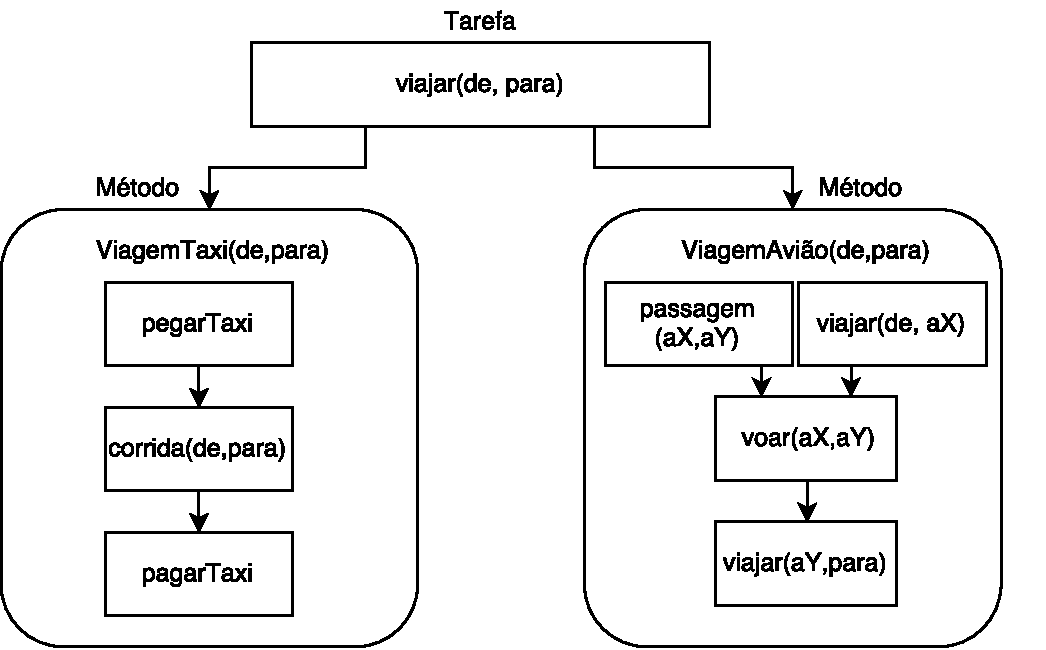
\includegraphics[width=0.8\textwidth]{fig/travelmethod.pdf}
	\caption{Exemplo de problema de HTN}
	\label{fig:travelmethods}
\end{figure}  

O planejamento HTN executa todas as possibilidades de resolução do problema, sempre respeitando a ordem dos métodos que conseguem ser realizados, quando um caminho de resolução leva a um fim de linha é realizado um retrocesso(\textit{backtracking}) até um caminho que tenha uma possibilidade de caminho diferente do que foi tomado anteriormente.

\subsection{AHTN} 

%AHTN é HTN + game tree search \cite{adversal}
\textit{Adversarial hierarchical-task network} (AHTN) é um algoritmo proposto para tentar solucionar o problema do grande fator de ramificação dos jogos em tempo real \cite{ontanon2015adversarial}. O algoritmo combina técnicas de planejamento HTN e o algoritmo \textit{minimax game tree search}. \\
%explicar Game search tree(minimax)
%explicar técnica de HTN utilizada
%explicar diferença do minimax puro

\subsection{Motivação e aplicação}
A motivação para o estudo de planejamento automatizado vem do fato que, como planejamento é um componente vital do comportamento racional, e a IA busca alcançar aspectos de inteligencia a nível computacional, então planejamento é um elemento chave para isso\cite{ghallab2004automated}.
%algumas aplicações de planejamento e exemplos

\section{Aprendizado} 
%-overview de aprendizado
%**O que é em geral \\
Para os humanos o aprendizado ocorre durante toda a vida. O aprendizado é o ato de adquirir novos conhecimentos, ou modificar conhecimentos já existentes ou ainda adquirir uma experiencia por repetição do ato de forma incorreta. Aprendizado pode variar de adquirir conhecimento de tarefas simples, como decorando um numero de telefone, até tarefas mais complicadas, como a formulação de novas teorias \cite{intelligence2003modern}. \\
Na computação o aprendizado depende de alguns fatores \cite{intelligence2003modern}:
\begin{itemize}
	\item Qual o conhecimento que será melhorado ou descoberto.
	\item Qual o conhecimento que o sistema já possui.
	\item Qual é a representação usada por esse conhecimento.
	\item Qual é o aprendizado disponível de fato.
\end{itemize}


\subsection{Aprendizado de Máquina} 

% o que é aprendizado de maquina
% Definição de ML: aprende atráves de um experiencia E em uma tarefa T com uma performace P  
% reinforcement o que é - aprendizado atráves de um conjunto de simulações
% explicar Q LEARNING

\subsection{Motivação e aplicação}
%motivação
%aplicação no mundo real com exemplos


%\section{Jogos Real-time Strategy(RTS)} 

%Jogos eletrônicos são muito populares, não só entre os jovens, principalmente pela grande quantidade de gêneros, existem jogos de ação, aventura, esportes, estrategia, entre outros. \\
%Dentro dos jogos de estratégia há uma subseção que se chama jogos de estratégia em tempo real, neles os jogadores estão se enfrentando no mesmo momento, como o nome já diz. Em alguns desses jogos há BOTs(jogadores que simulam um jogador real) e é preciso alguma inteligencia para esses BOTs conseguirem levar graça ao jogador real, para isso é utilizado algoritmos de IA. Esse tipo de jogo, devido a sua grande quantidade de ações, possui um fator de ramificação muito grande, e cresce exponencialmente, com isso aplicar os algoritmos se torna uma tarefa não trivial.  \\
%!TEX root = proposta.tex 
\chapter{\label{chap:obje}Objetivos}

Atualmente, há uma dificuldade na utilização de técnicas de IA para jogos em tempo real. Isso ocorre pelo fato que a IA precisa ser capaz de resolver tarefas, do mundo real, de maneira rápida e satisfatória. Geralmente, o espaço de estados dos jogos é enorme, isso faz com que não se tenha tempo de explorar todas as possibilidades de solução.   \\

%\frm{Seja mais específico, o que é difícil? Faltam técnicas?}

O intuito desse trabalho é mostrar que uma abordagem híbrida com planejamento e aprendizado de maquina pode ser uma alternativa valida para tratar esse gênero de jogo. 
%\frm{Não é bem a leitura de livros, tu vais te basear em um algoritmo específico que tu encontraste}
A leitura de livros será utilizada para adquirir embasamento teórico \cite{ghallab2004automated,intelligence2003modern,Mitchell1997ML} para entender as técnicas utilizadas no algoritmo AHTN \cite{ontanon2015adversarial}. Já a leitura dos artigos ajudará com a análise dos resultados \cite{ontanon2012experiments,hogg2010learning,ontanon2013survey}.
 \\ 
O jogo escolhido como plataforma foi o MicroRTS \cite{ontanon2013combinatorial}, pelo fato de que o jogo é uma simplificação de um jogo em tempo real, e é utilizado para demonstrar outras técnicas de IA . Como o jogo escolhido como plataforma já tem alguns algoritmos de IA implementados %\frm{Tu estás mencionando o jogo o qual tu ainda nem falou!!}
, a comparação com outros algoritmos pode ser considerado algo mais simples. %
%\frm{Talvez mover os objetivos para depois?} 

%\section{Objetivo Geral}

%O objetivo geral deste trabalho é implementar o algoritmo de planejamento AHTN \cite{ontanon2015adversarial} que combina técnicas de HTN com o algoritmo de \textit{minimax serach}. Após implementado, integrar aprendizado por reforço através da ferramenta WEKA\footnote{http://www.cs.waikato.ac.nz/ml/weka/} com o objetivo de melhorar o desempenho do algoritmo. Ao final do trabalho, o objetivo é conseguir comparar resultados obtidos com os resultados já publicados e consolidados \cite{ontanon2007case,ontanon2012experiments,hogg2010learning,buro2003real,ontanon2013survey}.  

\section{Objetivos Específicos}
\label{obj:esp}
\begin{itemize}
\item Estudar algoritmos de HTN.
\item Estudar o algoritmo de AHTN.
\item Estudar algoritmos de aprendizado por reforço.
\item Estudar como unir o algoritmo de AHTN com uma técnica de aprendizado por reforço. %\frm{E o AHTN? Te lembra que usamos aprendizado de máquina em minimax para compensar a falta de tempo para explorar tudo.}
\item Avaliar a aplicabilidade desses algoritmos junto ao jogo escolhido.
\item Definir a estratégia de implementação do algoritmo escolhido.
\item Comparar resultados com outras abordagens.
\end{itemize}



%\frm[inline]{De repente remover este objetivo}
%\section{Objetivo Adicional}

%Caso for possível atingir todos os objetivos propostos na seção \ref{obj:esp}, existe um item adicional %para aplicar a este trabalho:

%\begin{itemize}
%\item Testar o algoritmo em outro jogo RTS, como por exemplo Battle for Wesnoth\footnote{https://www.wesnoth.org/}\frm{Wesnoth não é RTS é um jogo de estratégia por turnos}.
%\end{itemize}

%%!TEX root = proposta.tex 
\chapter{\label{chap:descr}Descrição do Projeto}

\section{Algoritmo}
O algoritmo a ser implementado é o \textit{Adversarial hierarchical-task network} (AHTN). Nele são combinados técnicas de HTN com o algoritmo \textit{minimax search}. Após a implementação um algoritmo de aprendizado por reforço será incorporado para tentar melhorar o desempenho do algoritmo. O algoritmo \ref{alg:ahtn} é a representação da técnica de AHTN. Cada nodo da arvore das jogadas é definido por uma tupla $(s, N_{+}, N_{-}, t_{+}, t_{-})$, onde s é o estado corrente do ambiente, $N_{+}$ e $N_{-}$ são a representação de planos HTN para os jogadores max e min, respectivamente, $t_{+}$ e $t_{-}$ representam ponteiros para qual parte do plano HTN está sendo executado, sendo  $t_{+}$ uma tarefa de $N_{+}$ e $t_{-}$ uma tarefa de $N_{-}$. \textit{nextAction(N,t)} é uma função que, dado um HTN N e um ponteiro t, encontra a tarefa primitiva que deve ser executada em N. Se N ainda não estiver completamente decomposto, ou seja, ainda existem tarefas não primitivas, então \textit{nextAction(N,t)} = $\perp$    %\frm{Algoritmo o qual tu não falou nada ainda!! Aqui tu deixa muita coisa picando!}. 

\begin{algorithm}
	\caption{AHTNMax(s, $N_{+}$, $N_{-}$, $t_{+}$, $t_{-}$, d)}
	\label{alg:ahtn}
	\begin{algorithmic}[1]
		\If {terminal(s) $\vee$ d $\leq$ 0}
		\State	\Return ($N_{+}$, $N_{-}$, e(s))
		\EndIf
		\If {nextAction($N_{+}$, $t_{+}$) $\neq$ $\perp$}
		\State t = nextAction($N_{+}$, $t_{+}$) 
		\State \Return AHTNMin($\gamma$(s,t), $N_{+}$, $N_{-}$, t, $t_{-}$, d-1)
		\EndIf
		\State $N_{+}^{*}$ = $\perp$, $N_{-}^{*}$ = $\perp$, $v^{*}$ = $-\infty$
		\State $\aleph$ = $decompositions_{+}(s, N_{+}, N_{-}, t_{+}, t_{-})$
		\ForAll{$N \in \aleph$}
		\State $(N^{'}_{+}, N^{'}_{-}, v^{'}) = AHTNMax(s, N, N_{-}, t_{+}, t_{-}, d)$
		\If{$v^{'} > v^{*}$}
		\State $N_{+}^{*} = N^{'}_{+}, N_{-}^{*} = N^{'}_{-}, v^{*} = v^{'} $
		\EndIf
		\EndFor		
		\State \Return $(N_{+}^{*}, N_{-}^{*}, v^{*} )$
	\end{algorithmic}
\end{algorithm}

A grande diferença entre o algoritmo de AHTN e o algoritmo do \textit{minimax search}, é que as chamadas recursivas nem sempre se alternam entre max e min. O algoritmo troca de nodos max para min apenas quando os planos estão totalmente decompostos a ponto de gerar uma ação. 

\section{Ambiente}

%\frm[inline]{Remover os passivos}
%O ambiente que será utilizado é o MicroRTS. 
Utilizaremos o jogo MicroRTS como plataforma de teste para o algoritmo AHTN. O jogo MicroRTS foi feito por Santiago Ontañón \cite{ontanon2013combinatorial} para fins acadêmicos, com o intuito de aplicar e desenvolver técnicas de IA e para servir como prova de conceito para as técnicas criadas.  
O jogo é uma simplificação do jogo Starcraft\footnote{http://us.battle.net/sc2/pt/}. O jogo é um jogo RTS contra um adversário. O objetivo do jogo é destruir a base adversaria. Existem trabalhadores que podem coletar recursos e construir outros prédios. Os recursos são coletados dos minerais. Com os recursos é possivel construir bases de ataque, onde são realizado o treinamento de unidades de ataque. Para conseguir realizar o objetivo de destruir a base adversaria é preciso ter unidades de ataque. O jogo oferece três destas unidades, são elas:

\begin{itemize}
	\item Heavy - Possui um alto poder de ataque, mas sua velocidade é lenta.
	\item Light - Possui um baixo poder de ataque, mas sua velocidade é rapida.
	\item Ranged - Possui um ataque de longa distancia. 
\end{itemize} 

A Figura~\ref{fig:microrts}\footnote{https://github.com/santiontanon/microrts} mostra uma tela do jogo que representa o que foi explicado e ainda é possível observar que o fator de ramificação pode ser muito alto dependendo do cenário do jogo. %\frm{Figura sem explicação... Só os comentários do lado, em inglês, não te resolvem}

\begin{figure}[ht]
	\centering
	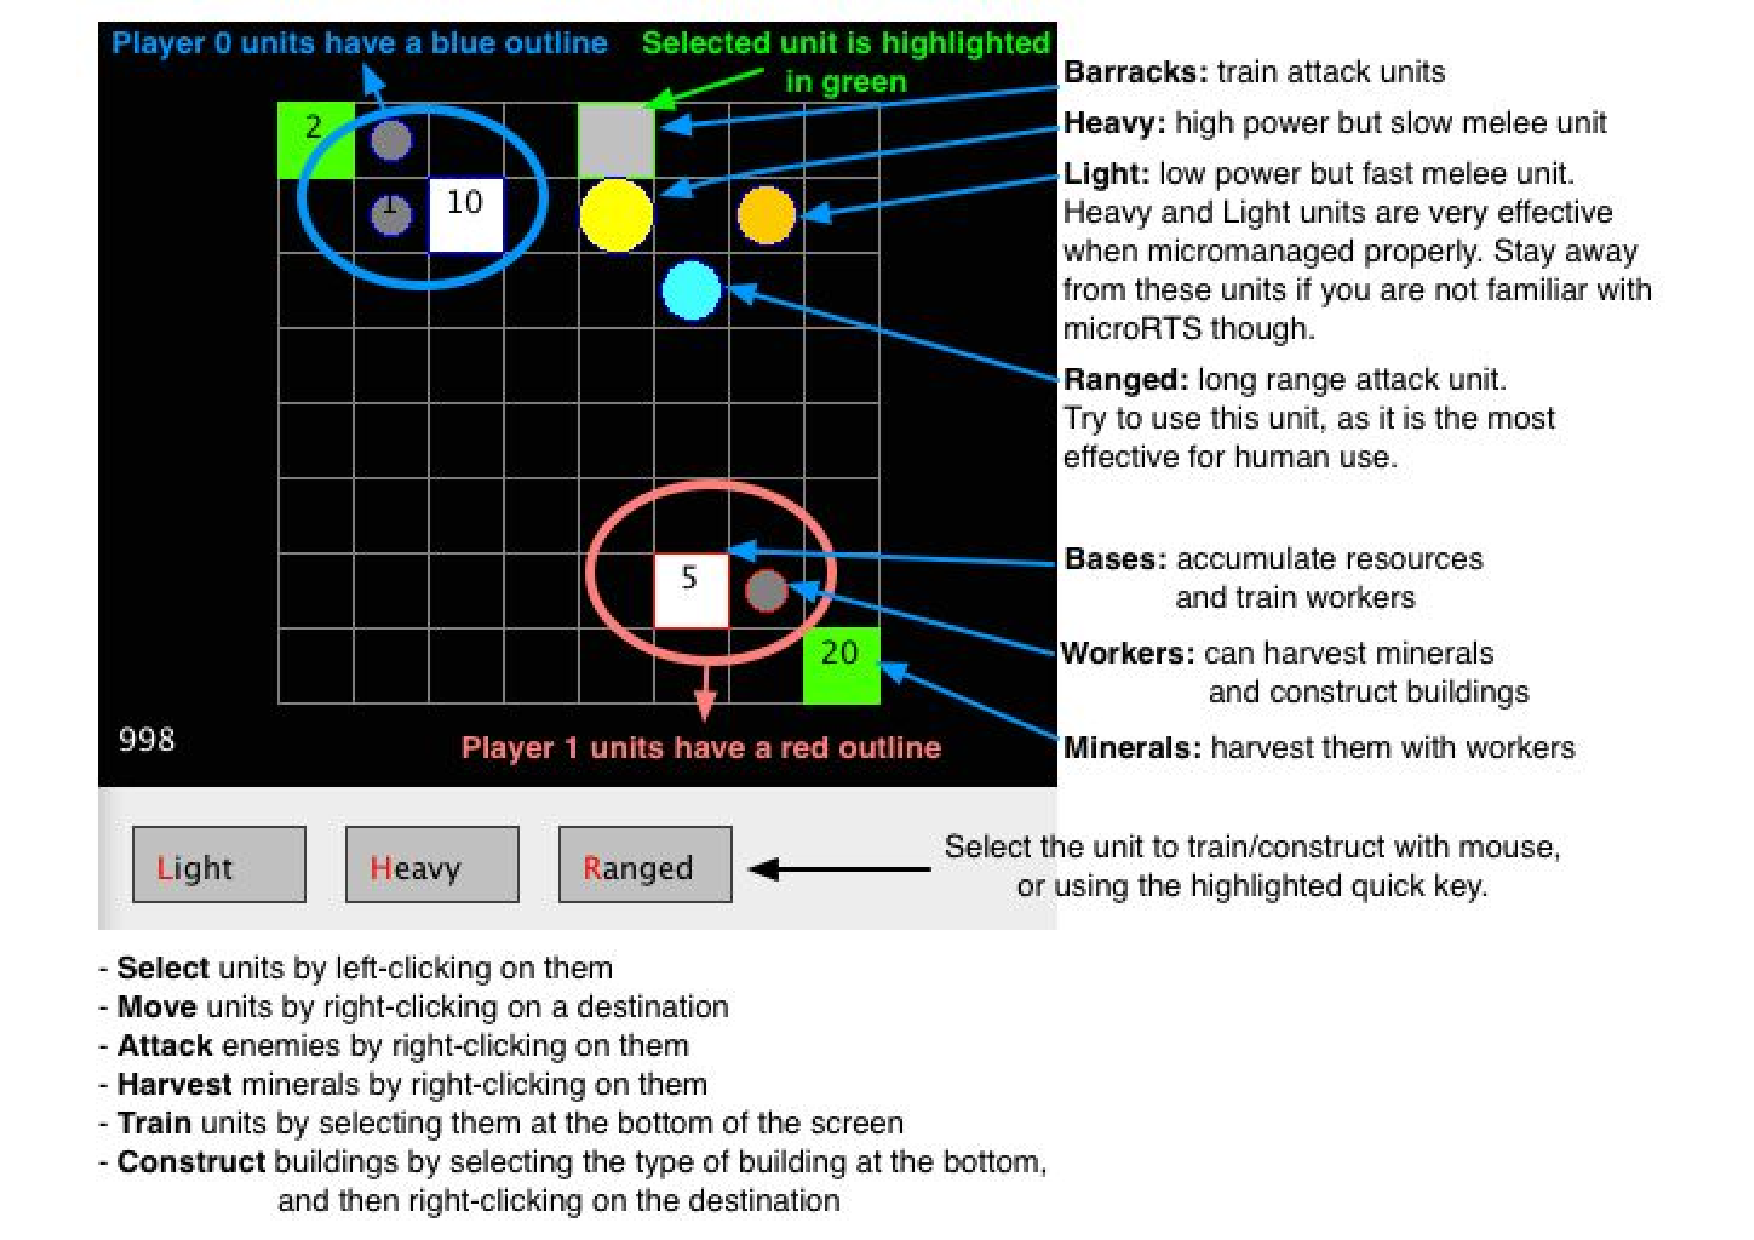
\includegraphics[width=0.8\textwidth]{fig/microrts.pdf}
	\caption{Uma foto da tela do MicroRTS}
	\label{fig:microrts}
\end{figure} 

No ambiente há algumas estrategias implementadas, cada estrategia possui variações dos algoritmos. Algumas das estrategias são:
\begin{itemize}
	\item Minimax Alpha-Beta Search Strategies - O que muda entre as técnicas é o jeito com que é feito a expansão do grafo.
	\item Monte Carlo Search Strategies - Executa jogadas aleatórias para planejar e após utiliza uma heurística para determinar em qual caminho seguir.
\end{itemize}

%\frm[inline]{E.. depois da itemização talvez seja interessante concluir algo}
A plataforma já foi utilizada para aplicar técnica de IA. Por esse motivo a utilização desta plataforma se torna viável. A comparação entre as estrategias já existentes com a que estou propondo pode mostrar que a abordagem resulta em um melhor desempenho. 

%!TEX root = volumeFinal.tex 
\chapter{\label{chap:ativ}Análise e Projeto}

\section{Jogos}
 Jogos eletrônicos são muito populares, principalmente pela grande quantidade de gêneros, existem jogos de ação, aventura, esportes, estratégia, entre outros. Hoje em dia, os jogos buscam que quem jogue consiga ficar imerso no dentro do jogo, sem conseguir identificar um padrão nos jogadores fictícios, pois se não o jogo deixa de ser tão interessante. Para que isso aconteça, a IA é associada a diversos jogos, e é comum pensar que quanto mais complexa a IA aplicada dentro do jogo mais difícil jogo irá ficar, mas isso nem sempre é verdade, nem sempre IA complicadas terão melhor desempenho do que as mais simples, uma boa IA dentro do jogo é feita a partir de determinar o comportamento certo para os algoritmo certos \cite{millington2009artificial}.
 
 \subsection{Jogos de estratégia em tempo real}
 
 Jogos de estratégia em tempo real, também conhecido por \textit{real-time strategy games} (RTS), é um subgênero de jogos de estratégia, onde os jogadores precisam construir uma base com uma economia, ganhando recursos, construindo edificações, treinando unidades de ataques e tecnologias para elas, tudo isso com o objetivo de destruir uma ou mais bases inimigas \cite{ontanon2013survey, buro2012real}. 
 
 Existem algumas diferenças entre jogos RTS e jogos de tabuleiro, como xadrez. Estas diferenças são \cite{ontanon2013survey}:
 
 \begin{itemize}
 	\item movimentos simultâneos, jogadores realizam jogadas ao mesmo tempo;
 	\item tempo real, cada jogador deve realizar suas ações em um curto espaço de tempo;
 	\item parcialmente observável, na maioria dos jogos RTS, o jogador só consegue enxergar parte do ambiente;
 	\item não-determinístico, nem sempre uma ação realizada resulta na saída esperada; e
 	\item complexidade, O espaço de estados e o número de ações possíveis é muito grande.
 \end{itemize} 
 
 
 Pelo fato de existirem essas diferenças, não é possível traduzir automaticamente as técnicas padrões dos jogos de tabuleiro para jogos RTS sem algum tipo de abstração ou simplificação \cite{ontanon2013survey}.
 
\subsection{MicroRTS}  
 
 Um exemplo deste gênero é o MicroRTS\footnote{https://github.com/santiontanon/microrts}, uma simplificação do jogo Starcraft\footnote{http://us.battle.net/sc2/pt/}, feita por Santiago Ontañón \cite{ontanon2013combinatorial} em Java. O MicroRTS foi desenvolvido para fins acadêmicos, com o intuito de aplicar e desenvolver técnicas de IA e para servir como prova de conceito para as técnicas criadas.
 
 \begin{figure}[ht]
 	\centering
 	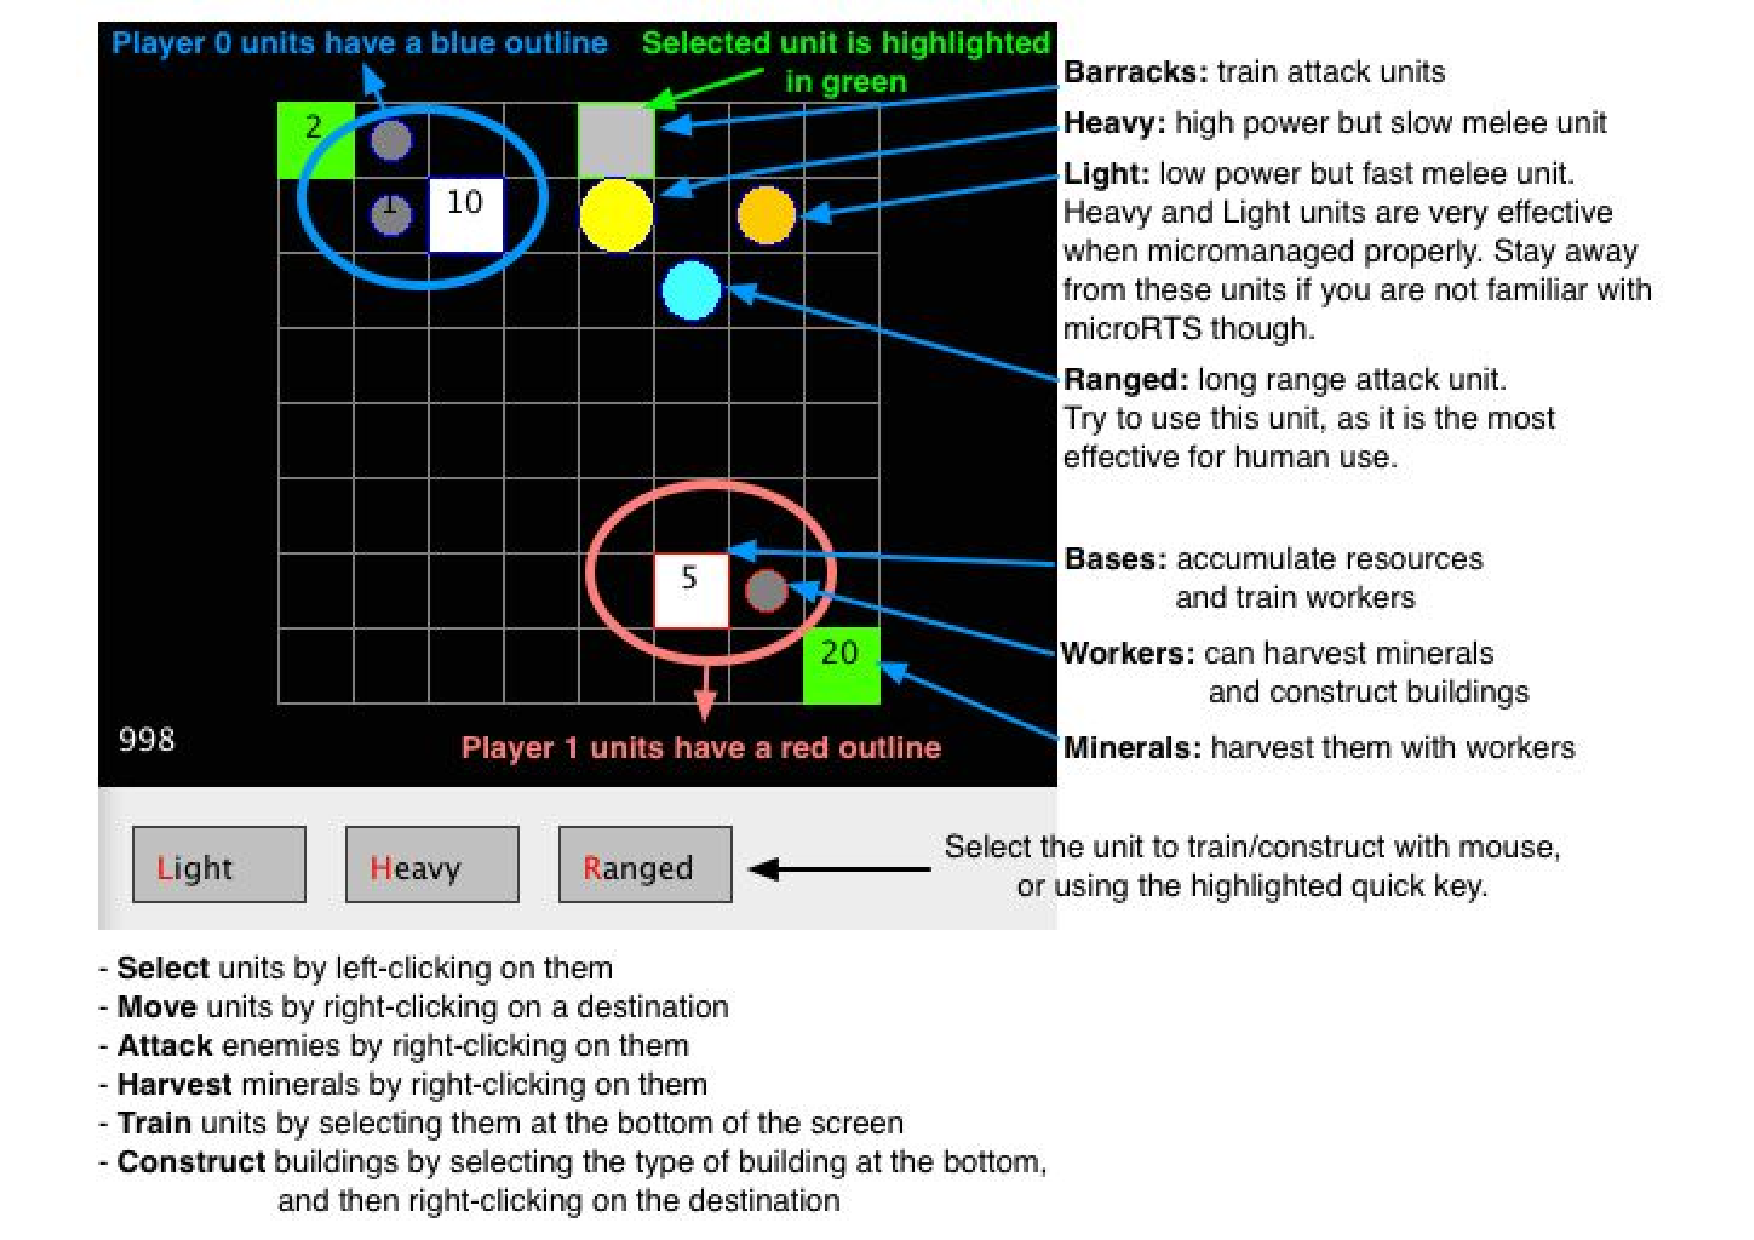
\includegraphics[width=0.5\textwidth]{fig/microrts.pdf}
 	\caption{Um exemplo de tela do MicroRTS}
 	\label{fig:microrts}
 \end{figure} 
 
O MicroRTS consiste em dois jogadores tentando destruir a base adversaria. Para destruir com o inimigo é preciso eliminar cada unidade e edificações adversarias. A Figura~\ref{fig:microrts} mostra uma tela do jogo. Existem quatro tipos de unidades no jogo, são elas:
  
\begin{itemize}
 	\item \textit{worker}, é responsável por coletar recursos e construir as edificações. Esta unidade também consegue lutar, mas possui um dano muito baixo;
 	\item \textit{heavy}, unidade que pode apenas atacar. Ela possui um alto poder de ataque, mas sua velocidade é lenta;
 	\item \textit{light}, unidade que pode apenas atacar. Ela possui um baixo poder de ataque, mas sua velocidade é rápida; e
 	\item \textit{ranged}, unidade que pode apenas atacar. Ela possui um ataque de longa distância. 
\end{itemize} 
 
Para adquirir as unidades é preciso das edificações e recursos. Existem três tipos de edificações, são elas:

\begin{itemize}
	\item base, a base é a edificação principal, ela é responsável pela criação dos \textit{workers}, e nela também é guardado os recursos coletados pelos \textit{workers};
	\item quartel, o quartel é responsável pela criação das unidades de ataque \textit{heavy}, \textit{light} e \textit{ranged}. Ela pode ser construída pelos \textit{workers} usando recursos; e
	\item base de recurso, na base de recurso são coletados os recursos pelos \textit{workers}, os a base de recursos é finitos para ser coletada.
\end{itemize}  

No início do jogo, cada jogador inicia com uma base, um \textit{worker} e uma base de recurso para coletar. Todas as unidades podem ser atacas menos a base de recursos. 
 
No ambiente há algumas estratégias implementadas, cada estratégia possui variações dos algoritmos. Algumas das estratégias são:
 \begin{itemize}
 	\item \textit{Minimax Alpha-Beta Search Strategies} - O que muda entre as técnicas é o jeito com que é feito a expansão do grafo.
 	\item \textit{Monte Carlo Search Strategies} - Executa jogadas aleatórias para planejar e após utiliza uma heurística para determinar em qual caminho seguir.
 \end{itemize}
 
 A plataforma já foi utilizada para aplicar técnica de IA. Por esse motivo a utilização dela se torna viável para a realização deste trabalho. 
Nela é possível observar que o fator de ramificação pode ser muito alto dependendo do cenário do jogo.

\subsection{Arquitetura do MicroRTS}

A arquitetura do MicroRTS é composta por 4 componentes principais: O Jogo em si, onde são feitas todas as ações dos jogos. As unidades, onde todas as ações de cada unidade podem ser controladas e acessadas, por exemplo, saber onde está cada unidade inimiga. A Interface gráfica, responsável pela representação gráfica do jogo. E a Inteligência Artificial, onde pode ser acoplado a IA que desejar, a plataforma já possui algumas como foi dito anteriormente. A imagem \ref{fig:pacotes} representa os componentes.

 \begin{figure}[ht]
 	\centering
 	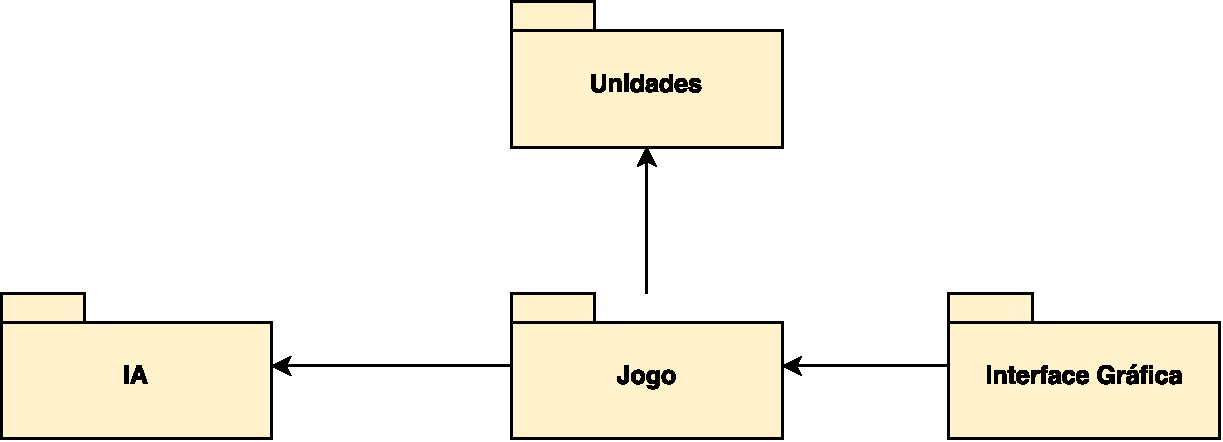
\includegraphics[width=0.7\textwidth]{fig/pacotes.pdf}
 	\caption{Arquitetura MicroRTS}
 	\label{fig:pacotes}
 \end{figure} 
 
\section{Descrição do Projeto}
 
Para realizar a implementação de uma IA para acoplar no MicroRTS, é preciso conhecer as classes responsáveis por cada componente. A imagem \ref{fig:classes} apresenta, as classes principais. A Classe \textit{GameVisualSimulation} é a interface entre os componentes do jogo e o usuário. A classe \textit{GameState} e \textit{PhysicalGameState}, são responsáveis pelo controle das ações das unidades, e pelo controle do mapa e das unidades dentro dele, respectivamente. A classe \textit{UnitTypeTable} é onde cada unidade é associada as ações possíveis no jogo. A Classe \textit{PhysicalGameStatePanel} é responsável pela interface gráfica. E por fim a classe \textit{AHTN} é onde minha proposta de solução será acoplada ao jogo.
 
  \begin{figure}[ht]
  	\centering
  	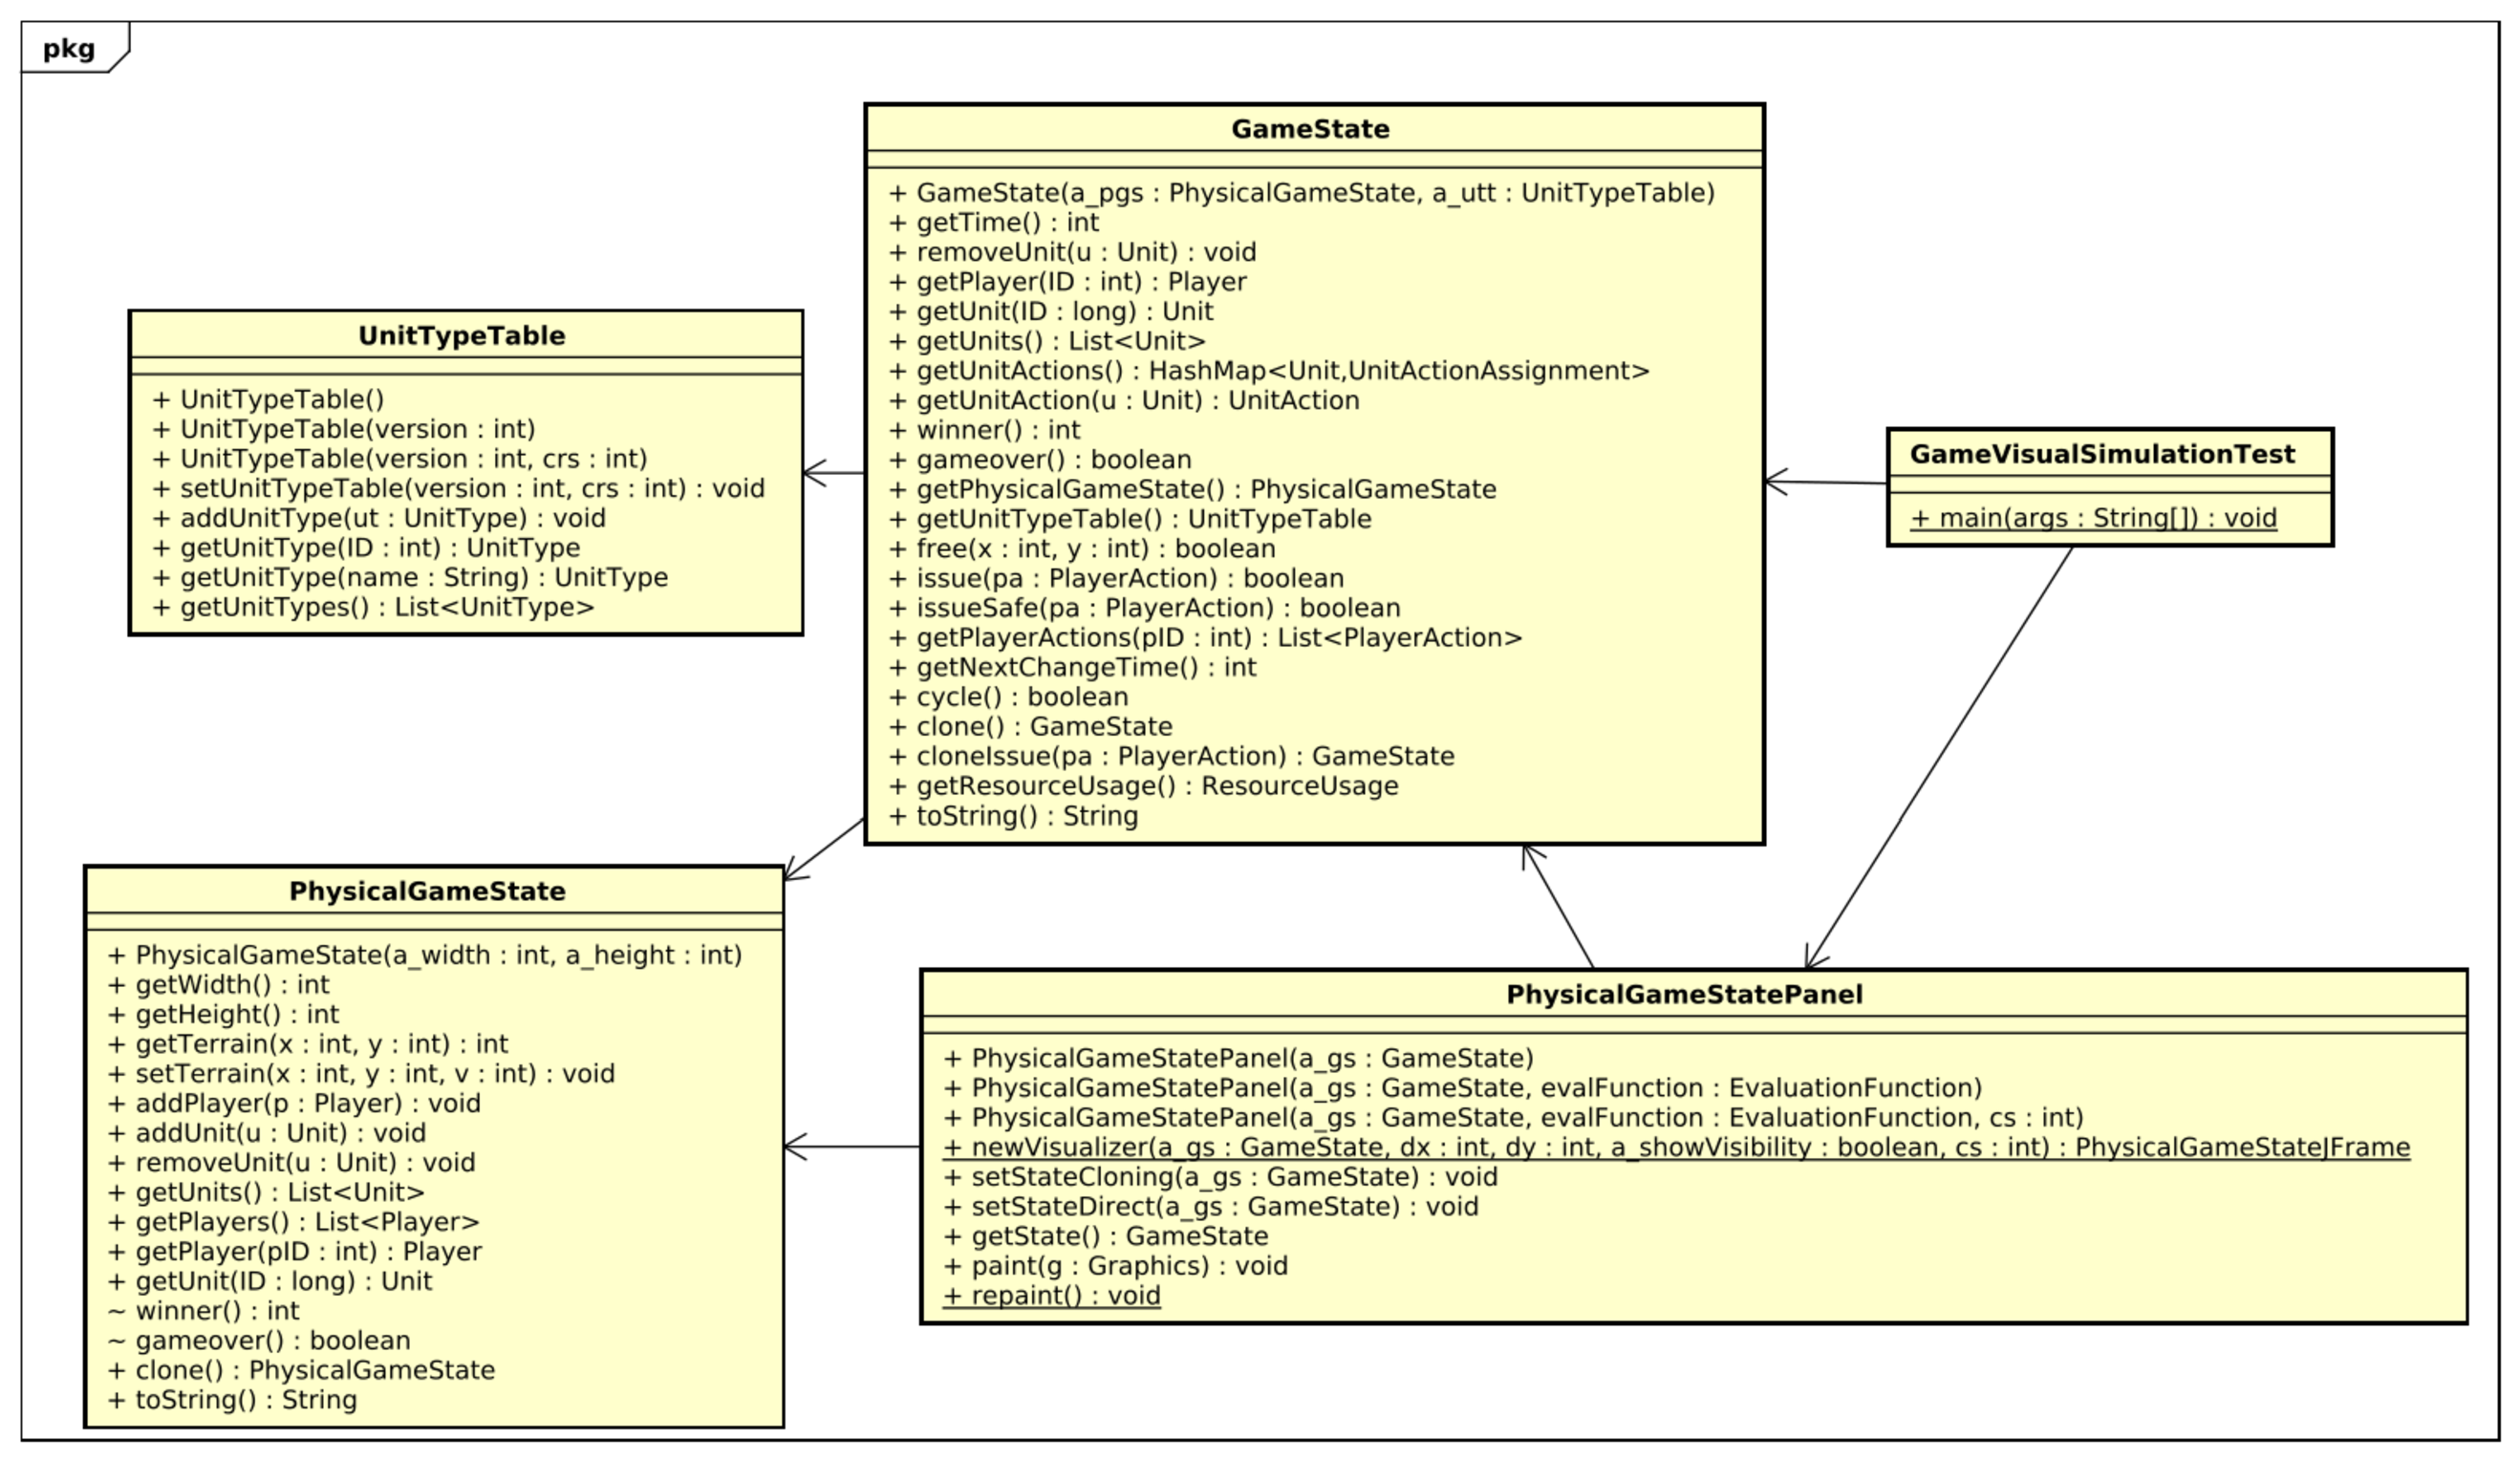
\includegraphics[width=0.7\textwidth]{fig/classes.pdf}
  	\caption{Classes do MicroRTS}
  	\label{fig:classes}
  \end{figure} 


\section{Cronograma}

Para a próxima etapa do projeto do Trabalho de Conclusão, foi proposto o plano das atividades apresentado no diagrama de Gantt com a respectiva legenda.

\begin{itemize}
\item Tarefa 1 - Escrita do TC II.
\item Tarefa 2 - Desenvolvimento do dominio.
\item Tarefa 3.1 - Implementação do algoritmo AHTN.
\item Tarefa 3.2 - Testar e corrigir possíveis erros da implementação.
\item Tarefa 4 - Criação dos \textit{benchmark}.
\item Tarefa 5 - Integrar o algoritmo de \textit{q-learning} a implementação. 
\item Tarefa 6 - Realizar a comparação com as outras abordagens. 
\item Tarefa 7 - Preparar a apresentação. 
\end{itemize}

\begin{ganttchart}{1}{21}
	\gantttitle{Volume Final TCI}{21} \\
	\gantttitlelist{6,...,12}{3} \\
	\ganttgroup{TC II}{6}{20} \\	
	\ganttmilestone{Entrega do volume Final TCI}{3} \ganttnewline	
	\ganttbar{Tarefa 1}{7}{20} \\	
	\ganttbar{Tarefa 2}{7}{8} \\
	\ganttbar{Tarefa 3.1}{9}{10} \\	
	\ganttbar{Tarefa 3.2}{11}{12} \\	
	\ganttbar{Tarefa 4}{13}{14} \\
	\ganttbar{Tarefa 5}{15}{16} \\
	\ganttbar{Tarefa 6}{17}{18} \\	
	\ganttbar{Tarefa 7}{19}{20} \\	
	\ganttmilestone{Entrega Volume Final}{20} \ganttnewline
	%\ganttlinkedgroup{Task 3}{2}{3}
	%\ganttlinkedbar{Task 3}{3}{7} \ganttnewline
%	%\ganttmilestone{Milestone}{7} \ganttnewline
%	%\ganttbar{Final Task}{8}{12}	
%	\ganttlink{elem2}{elem8}
%	\ganttlink{elem5}{elem6}	
%	\ganttlink{elem3}{elem6}
%	\ganttlink{elem4}{elem7}
%	\ganttlink{elem6}{elem7}
%	\ganttlink{elem8}{elem9}
\end{ganttchart}



%----------------------------------------------------------------
% Aqui vai a bibliografia. Existem 3 estilos de citação: use
% 'tcc-alpha' para citações do tipo [Abc+] ou [XYZ] (em ordem
% alfabética na bibliografia), 'tcc-num' para citações
% numéricas do tipo [1], [20], etc., em ordem de referência e
% 'tcc-alpha-full' para citações estilo 'alpha' mas com nomes completos.
%----------------------------------------------------------------
%\bibliographystyle{tcc-alpha}
%\frm[inline]{A citação para o Russel e Norvig está errada, para que o título é o autor!!}
\bibliographystyle{tcc-num}
\bibliography{referencias}

%----------------------------------------------------------------
% Após \appendix, se iniciam os capítulos de Apêndice, com
% numeração alfabética.
%----------------------------------------------------------------
%\appendix
%\chapter{Meu primeiro apêndice}
%\chapter{My second appendix}

%----------------------------------------------------------------
% Aqui vão os "capítulos" de anexos. Cada anexo deve
% ser considerado um capítulo.
%----------------------------------------------------------------
%\anexos
%\chapter{Meu primeiro anexo}
%\chapter{My second attachment}

% E aqui (para a felicidade de todos) termina o documento.
\end{document}
